\chapter{Background}
\label{chap:background}
Engineered systems often come with conditions for operation -- televisions and phones are rated for use only in a range of temperature values, and voltage standards, beyond which they can malfunction.
Machine learning models are no different -- they operate under a set of assumptions about the inputs.
These assumptions are critical when machine learning models encounter variations in inputs at test time or during deployment.
This chapter contains an overview of existing techniques that have been designed to overcome challenges in machine learning that are encountered as a result of deviations between training and test distributions.
In this chapter, we will review literature on robust machine learning, and relevant work in image classification and visual question answering, which will serve as a starting point for subsequent chapters.

\section{Robust Machine Learning}

\subsection{What is Robustness?}
Robustness is an overloaded word in machine learning and is often used with inconsistent connotations by different researchers.
Before we get into the math, it makes sense to develop a simple intuitive definition that we will stick with in this dissertation.
This simple definition is as follows:  machine learning models are trained on a certain dataset but may encounter different types of changes at test time and with varying degrees -- a robust machine learning model is able to reliably produce outputs irrespective of such changes in inputs.
When these changes are designed (either by humans or by algorithms) to fool the model into making incorrect predictions, we will denote such inputs as adversarial examples; the property of a model which is robust under such circumstances will be denoted as \textit{``adversarial robustness''}.
When the entire input distribution shifts in meaningful ways (for instance, grayscale images vs.~color images, or photos vs.~sketches), we will denote this as domain shift, and the property of models that are robust to such shifts as \textit{``domain generalization''.}



Consider a training distribution $P_{tr}$ consisting of inputs $\x$ and labels $\y$.
Under the empirical risk minimization (ERM), the following risk is minimized:
\begin{equation}
    \mathcal{R}_{ERM} = \E_{(\x, \y) \sim P_{tr}}  ~\ell(f(\x; \theta), \y).
    \label{eq:erm}
\end{equation}
ERM provides generalization guarantees~\citep{vapnik1991principles} for i.i.d.\ test samples, but not for out-of-distribution or adversarial examples~\citep{biggio2013evasion,szegedy2014intriguing}. 

\paragraph{Distributed Robust Optimization (DRO)}~\citep{pmlr-v80-hu18a,sagawa2020distributionally} searches for loss-maximizing perturbations of the input within an $\epsilon$-divergence ball around $P_{tr}$ and minimize the risk over such perturbed distributions.
\begin{equation}
    \mathcal{R}_{DRO}=\underset{P:D(P, P_{tr})<\epsilon}{sup}\E_{(\x, \y) \sim P} \ell(f(\x; \theta), \y).
    \label{eq:std_adv}
\end{equation}
The solution to Equation~\ref{eq:std_adv} guarantees robustness inside such $\epsilon$-bounded distributions $P$.
The inner maximization is typically solved using gradient-based methods~\citep{madry2018towards} over additive perturbations $\delta$ such that $\x+\delta$ fools the classifier.

\paragraph{Adversarial Examples.}

% Much of our discussion will revolve around an optimization view of adversarial
% robustness. This perspective not only captures the phenomena we want to study in
% a precise manner, but will also inform our investigations. 
% To this end, let us
% consider a standard classification task with an underlying data distribution $\D$ 
% over pairs of examples $x \in \R^d$ and corresponding labels $y \in [k]$. We also
% assume that we are given a suitable loss function $\loss(\theta, x, y)$, for instance the
% cross-entropy loss for a neural network. As usual, $\theta \in \R^p$ is the set of
% model parameters. Our goal then is to find model parameters $\theta$ that minimize
% the risk $\E_{(x, y) \sim \D}[\loss(x, y, \theta)]$.


% Empirical risk minimization (ERM) has been tremendously successful as a recipe
% for finding classifiers with small population risk. Unfortunately, ERM often
% does not yield models that are robust to adversarially crafted examples
% \citep{biggio2013evasion,szegedy2014intriguing}. 
% Formally, there
% are efficient algorithms (``adversaries'') that take an example $x$ belonging
% to class $c_1$ as input and find examples $x^\adv$ such that $x^\adv$ is very
% close to $x$ but the model incorrectly classifies $x^\adv$ as belonging to
% class $c_2 \neq c_1$.

% In order to \emph{reliably} train models that are robust to adversarial attacks,
% it is necessary to augment the ERM paradigm appropriately.  Instead of resorting
% to methods that directly focus on improving the robustness to specific attacks,
% our approach is to first propose a concrete \emph{guarantee} that an
% adversarially robust model should satisfy. We then adapt our training methods
% towards achieving this guarantee.

To formally define adversarial examples, first an \emph{attack model} is specified -- this provides a precise definition of the input perturbations that we want robustness against.
Given an input $x$, we define this set of allowed perturbations $\hood \subseteq \R^d$.
For image classification, 
$\hood$ is typically chosen to be the $\ell_\infty$-ball around $x$~\citep{goodfellow2014explaining}. 
Defense against is formulated by \citet{madry2018towards} as a min-max optimization, where the inner maximization allows the attack model to maximally fool the classifier, and the outer minimization of the classifier loss uses the resulting adversarial examples to update model parameters.
\begin{equation}
\label{eq:minmax}
	\min_\theta \rho(\theta),\quad \text{ where }\quad \rho(\theta) =
    \mathbb{E}_{(x,y)\sim\mathcal{D}}\big[\max_{\delta\in 
    \hood}
    \ell(\theta,x+\delta,y)\big] \; .
\end{equation}

\textbf{Domain Generalization}
has been explored under both multi-source (MSDG) and single-source (SSDG) settings. Techniques designed for MSDG seek to utilize the multiple domains to perform feature fusion~\citep{shen2019situational}, learning domain-invariant features~\citep{ganin2016domain}, meta-learning~\citep{li2018learning}, invariant risk minimization~\citep{arjovsky2019invariant}, learning mappings between multiple training domains~\citep{robey2021model}, and style randomization~\citep{nam2021reducing}.
Gulrajani  \textit{et al.}~\citep{gulrajani2021in} provide an extensive comparative study of these approaches and report that simply performing ERM on the combination of source domains leads to the best performance. Many benchmarks have been proposed to evaluate MSDG performance such as PACS~\citep{li2017deeper}, OfficeHome~\citep{venkateswara2017deep}, Digits~\citep{volpi2018generalizing}, and WILDS~\citep{koh2021wilds} which is a compendium of MSDG datasets for various tasks such as image classification, text sentiment classification, text toxicity prediction, etc. In the context of multi-source DG, \citep{zhou2020learning} propose to synthesize novel domains using a conditional generator trained on multiple domains using cycle consistency -- whereas we are primarily interested in the single source setting where such a method may not be feasible. Moreover, we strictly synthesize novel domains as functions of the source domain, and place emphasis on the nature of functions that are learnable during training with a convolutional network with objectives such as an adversarial cost and consistency measures.

SSDG is a harder setting due to the lack of multiple datasets for using the above methods; most work in SSDG has therefore focused on data augmentation.
Notable among these methods is the idea of adversarial data augmentation -- ADA\citep{volpi2018generalizing} and M-ADA~\citep{qiao2020learning} apply pixel-level additive perturbations to the image in order to fool the classifier.  Resulting images are used as augmented data to train the classifier.
% is trained over the union of source dataset and adversarial samples.
RandConv~\citep{xu2020robust} shows that shape-preserving transformations in the form of random convolutions of images lead to impressive performance gains on Digits.
% benchmark.

\textbf{Robustness to Image Corruptions.}
There has also been interest in training classifiers that are robust to corruptions that occur in the real world, such as different types of noise and blur, artifacts due to compression techniques, and weather-related environments such as fog, rain, and snow.
\citep{vasiljevic2016examining,geirhos2018generalisation} show that training models with particular types of corruption augmentations does not guarantee robustness to other unseen types of corruptions or even different severities of corruptions. 
Hendrycks~ \textit{et al.}~\citep{hendrycks2018benchmarking} curate benchmarks (ImageNet-C and CIFAR-C) to test robustness along a fixed set of corruptions.
They also provide a benchmark called ImageNet-P which tests robustness against other corruption types such as small tilts and changes in brightness.
A similar benchmark for corruptions of handwritten digit images, MNIST-C~\citep{mu2019mnist} has also been introduced.

% \paragraph{Robustness to Adversarial Attacks}




\section{Robust Natural Language Understanding}
Generation of semantics-preserving adversarial examples 
\citep{jia2017adversarial,ribeiro2018semantically,iyyer2018adversarial,alzantot2018generating}, and approaches to defend against word substitution~\citep{jia2019certified} have been explored.
Evaluation datasets have also been proposed for textual entailment that are manually crafted~\citep{gardner2020evaluating} or template-based~\citep{mccoy2019right,glockner2018breaking,naik2018stress}.
\citet{belinkov2018synthetic,ebrahimi2018hotflip,jones2020robust} investigate the practical problem of typographical errors in NLP systems.
While humans seem to understand most spelling or grammar errors when presented with context, this is not true for existing NLP systems.
\citet{zhao2017men,hendricks2018women,rudinger2018gender} show that NLP systems can propagate and amplify socio-cultural biases.
\citet{jia-etal-2019-certified} have shown how interval bound propagation~\citep{dvijotham2018dual} can be used to defend text classification models from adversarial word substitutions.
Inspired by the work on adversarial training in computer vision, several optimization strategies have been developed for fine-tuning pre-trained language models~\citep{miyato2016adversarial,oren2019distributionally,jiang2020smart,zhu2020freelb}.

\section{Robustness and Generalization in Vision and Language}
\begin{figure}[t]
    \centering
    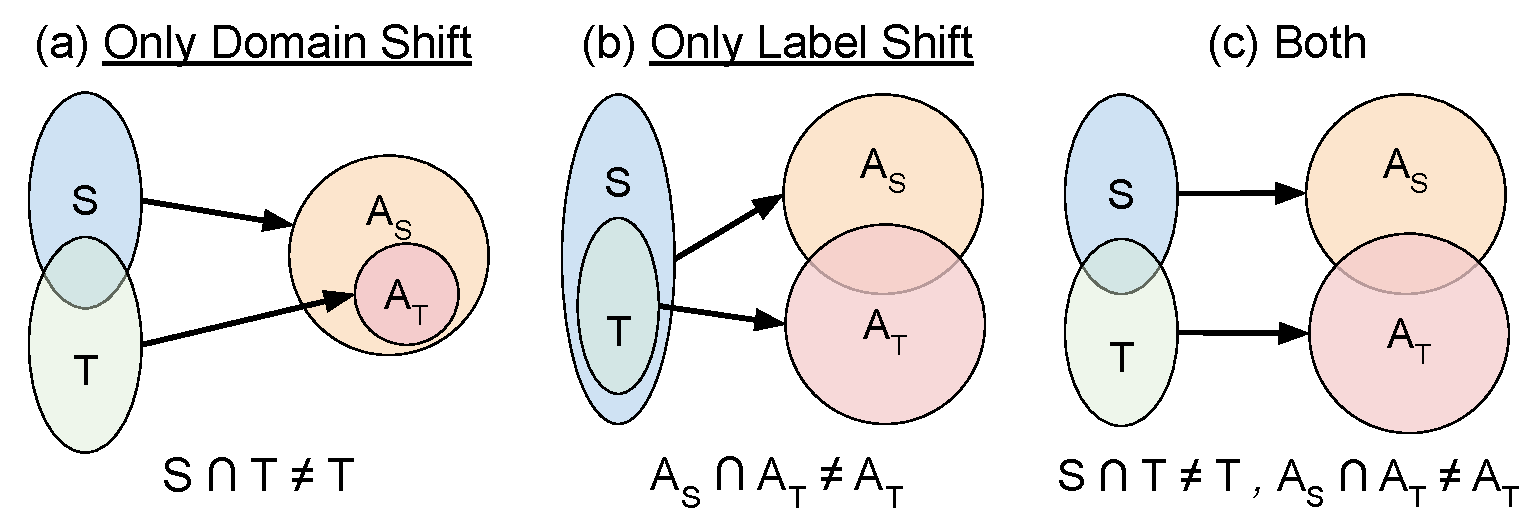
\includegraphics[width=\linewidth]{figures/generalization_types.pdf}
    \caption{Aspects of generalization in VQA.}
    \label{fig:generalization_types}
\end{figure}
The presence of two modalities in V\&L tasks implies that we need to talk about robustness and generalization of V\&L modalities from the perspective of vision, and from the perspective of language.
Most of the robustness literature in V\&L has been for the task of visual question answering.
We review it below.

Robustness in VQA can be defined as shown in Figure~\ref{fig:generalization_types} under two situations: domain shift and label shift.
Under domain shift, generalization to a new input domain (such as different styles of questions or novel scenes) is desired, characterized by $S\cap T \neq T$ where $S$ and $T$ denote the train and test input domains.
Under label shift, generalization to novel answers is desired (predicting answers not seen during training), characterized by $A_S\cap A_T \neq A_T$, where $A_S$ and $A_T$ are the set of answers seen during training and test-time.

Performance under \textbf{domain shift} has been evaluated for new domains of test questions with unseen words and objects~\citep{teney2016zero,ramakrishnan2017empirical}, 
novel compositions~\citep{johnson2017clevr,agrawal2017c}, 
logical connectives~\citep{gokhale2020vqa}, as well as questions that are
implied~\citep{ribeiro-etal-2019-red}, entailed~\citep{ray2019sunny} or sub-questions~\citep{selvaraju2020squinting}; or for datasets with varying linguistic styles~\citep{chao2018cross,xu2019open,shrestha2019answer}
and different reasoning capabilities~\citep{kafle2017analysis}.
Other work seeks to answer target questions that are sub-questions~\citep{selvaraju2020squinting}, or are implied~\citep{ribeiro-etal-2019-red} or entailed~\citep{ray2019sunny} by source questions.
More recently, a new benchmark has been proposed that combines many of the papers mentioned above into a unified evaluation dataset for testing robustness of VQA models~\citep{li2020closer}.


\textbf{Label shift} or Prior Probability Shift~\citep{storkey2009training} has been implicitly explored in VQA-CP~\citep{agrawal2018don}, where the conditional probabilities of answers given the question type deviate at test-time.
% are designed to be different for the train and test shifts.
% \citet{teney2020value} have identified several pitfalls associated with the models and evaluation criteria for VQA-CP.
A similar benchmark for the spatial visual question answering task has been introduced via GQA-OOD~\citep{kervadec2020roses}, which focuses on rare question-answer pairs, and showed that existing VQA models overfitted to dataset biases and underperformed on such OOD questions. 
Similar to GQA-OOD, the VQA-CE dataset~\citep{dancette2021beyond} generated a new evaluation set by using rules to mine questions that can fool existing models.
As for GQA-OOD, this dataset demonstrated that SOTA
models do not perform well when they can’t rely on shortcuts, even models which use bias-reduction
techniques. 
A comprehensive survey of methods that tackle such dataset biases and priors is given by \citet{shrestha2022investigation} and \citet{teney2020value}.





% Approaches such as~\citet{RUBI,teney2019actively,teney2020unshuffling,chen2020counterfactual,gokhale2020mutant} have been recently proposed as solutions to the VQA-CP challenge.
% In the VQA-v2 dataset~\citep{goyal2017making}, questions are created for each image $i \in \mathcal{I}$ by human workers, and the test-train splits are i.i.d. with respect to question-type, and for each question, two images leading to two different answers are collected.
% This is an example of neither domain shift nor label shift.

